\documentclass[tikz,border=4pt]{standalone}
\usepackage{amsmath}
\begin{document}
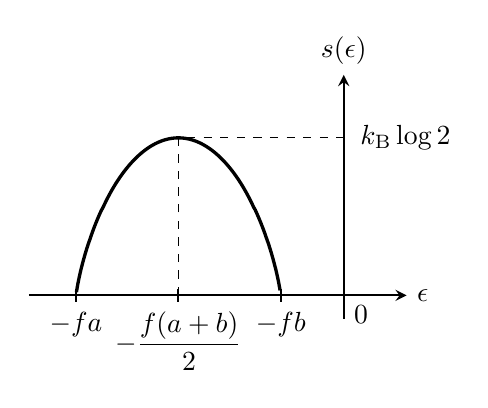
\begin{tikzpicture}[>=stealth, thick, scale=1.0]
  % Axes: epsilon in [-fa, -fb], mapped to x in [-3.4, -0.8]
  \draw[->] (-4.0, 0) -- (0.8, 0) node[right] {$\epsilon$};
  \draw[->] (0, -0.3) -- (0, 2.8) node[above] {$s(\epsilon)$};
  \node[below right] at (0, 0) {$0$};

  % Binary entropy dome on [-3.4, -0.8], midpoint -2.1, width 2.6
  % s = - (p*ln(p) + (1-p)*ln(1-p)) / ln(2) * 2.0
  \draw[very thick, domain=0.002:0.998, samples=140]
    plot ({-3.4 + 2.6*\x}, {-2.0 * (\x*ln(\x) + (1-\x)*ln(1-\x)) / ln(2)});

  % Ticks and labels
  \draw (-3.4, 0.08) -- (-3.4, -0.08) node[below] {$-fa$};
  \draw (-2.1, 0.08) -- (-2.1, -0.08) node[below] {$-\dfrac{f(a+b)}{2}$};
  \draw (-0.8, 0.08) -- (-0.8, -0.08) node[below] {$-fb$};

  % Max value k_B log 2
  \draw[dashed, thin] (-2.1, 0) -- (-2.1, 2.0) -- (0, 2.0);
  \node[right] at (0.08, 2.0) {$k_{\mathrm{B}}\log 2$};
\end{tikzpicture}
\end{document}
